%
% Portuguese-BR vertion
% 
\documentclass{report}

\usepackage{ipprocess}
% Use longtable if you want big tables to split over multiple pages.
\usepackage{longtable}
\usepackage{tikz}
\usepackage[utf8]{inputenc}
\usepackage[brazil]{babel} % Uncomment for portuguese
\usepackage{pdflscape} % set ladscape/portrait pdf pages

\sloppy

\graphicspath{{./pictures/}} % Pictures dir
\makeindex

\begin{document}

\DocumentTitle{Documento de Arquitetura}
\Project{Core-MUSA}
\Organization{Universidade Estadual de Feira de Santana}
\Version{Build 3.0}

\capa

%%%%%%%%%%%%%%%%%%%%%%%%%%%%%%%%%%%%%%%%%%%%%%%%%%
%% Revision History
%%%%%%%%%%%%%%%%%%%%%%%%%%%%%%%%%%%%%%%%%%%%%%%%%%
\chapter*{Histórico de Revisões}
\begin{center}
	\begin{longtable}[pos]{|m{2cm} | m{8cm} | m{4cm}|} 
		\hline
		\cellcolor[gray]{0.9}
		\textbf{Date} & \cellcolor[gray]{0.9}\textbf{Descrição} & \cellcolor[gray]{0.9}\textbf{Autor(s)}\\ \hline
		\endfirsthead
		\hline
		\multicolumn{3}{|l|}%
		{{\bfseries continuação da página anterior}} \\
		\hline
		\cellcolor[gray]{0.9}
		\textbf{Date} & \cellcolor[gray]{0.9}\textbf{Descrição} & \cellcolor[gray]{0.9}\textbf{Autor(s)}\\ \hline
		\endhead
		
		\multicolumn{3}{|r|}{{continua na próxima página}} \\ \hline
		\endfoot
		
		\hline
		\endlastfoot
		
		20/10/2014 & Concepção do documento & fmbboaventura \\ \hline
		23/10/2014 & Revisão inicial & jadsonfirmo \\ \hline
		29/10/2014 & Foi adicionada uma breve descrição dos componentes & fmbboaventura \\ \hline       
		29/10/2014 & \textit{Stakeholders} & jadsonfirmo \\ \hline
		30/10/2014 & Ajustes estruturais & fmbboaventura e jadsonfirmo \\ \hline
		30/10/2014 & Detalhamento das instruções & jadsonfirmo, KelCarmo e Odivio \\ \hline
		30/10/2014 & Adição dos diagramas de classe & gordinh \\ \hline
		06/11/2014 & Mudanças nos \textit{layouts} das instruções e no diagrama de classe da ULA & jadsonfirmo e KelCarmo \\ \hline
		10/11/2014 & Detalhamento dos opcodes & jadsonfirmo \\ \hline
		13/11/2014 & Alteração na tabela dos opcodes & jadsonfirmo \\ \hline
		17/11/2014 & Alteração no diagrama de classe da ULA e ajustes na tabela de opcodes & jadsonfirmo \\ \hline
		18/11/2014 & Ajuste dos opcodes & jadsonfirmo \\ \hline
		24/11/2014 & Refatoração do \textit{Datapath} & Odivio Caio \\ \hline
		07/12/2014 & Opcodes de acordo com o \textit{software} Vênus & jadsonfirmo \\ \hline
		07/12/2014 & Alteração no \textit{layout} do JR e remoção de conflitos & jadsonfirmo \\ \hline
		09/12/2014 & Correções estruturais do documento & di3goleite \\ \hline
		11/12/2014 & Revisão & jadsonfirmo \\ \hline
		12/12/2014 & Correção de bug na tabela de Busca de Registradores & di3goleite \\ \hline
		15/12/2014 & Correção do datapath no documento e da tabela de histórico de revisões & di3goleite \\ \hline
		15/12/2014 & Revisão da visão geral da arquitetura & di3goleite \\ \hline
		15/12/2014 & Correção dos OPCODES do JR e do SUBi & di3goleite \\ \hline
		16/12/2014 & Mudanças no datapath e descrição da arquitetura & di3goleite \\ \hline
		17/12/2014 & Finalização da descrição da arquitetura & di3goleite \\ \hline
		17/12/2014 & Revisão parcial do documento e das definições de entrada e saídas &gordinh \\ \hline
	\end{longtable}
\end{center}

% TOC instantiation
\tableofcontents

%%%%%%%%%%%%%%%%%%%%%%%%%%%%%%%%%%%%%%%%%%%%%%%%%%
%% Document main content
%%%%%%%%%%%%%%%%%%%%%%%%%%%%%%%%%%%%%%%%%%%%%%%%%%
\chapter{Introdução}
  
  \section{Propósito do Documento}
  Este documento descreve a arquitetura do projeto \ipPROCESSProject, incluindo as especificações dos circuitos internos, bem como suas devidas máquinas de estados. Também, serão apresentados diagramas de classes, de temporização e definições de entradas e saídas. O principal objetivo deste documento é definir as especificações de arquitetura do \ipPROCESSProject \space e provê uma visão geral do projeto.
  
  \section{Stakeholders}
    \FloatBarrier
    \begin{table}[H] 
      \begin{center}
        \begin{tabular}[pos]{|m{6cm} | m{8cm}|} 
          \hline 
          \cellcolor[gray]{0.9}\textbf{Nome} & \cellcolor[gray]{0.9}\textbf{Papel/Responsabilidades} \\ \hline
           Diego Leite e Lucas Morais & Gerência  \\ \hline
           Victor Figueiredo, Matheus Castro, Odivio Caio Santos e Kelvin Carmo & Desenvolvimento  \\ \hline
           Filipe Boaventura e Wagner Bittencourt & Implementação  \\ \hline
           Jadson Firmo & Análise e refatoração  \\ \hline
        \end{tabular}
      \end{center}
    \end{table} 

\section{Visão Geral do Documento}

Este documento é dividido através dos seguintes capítulos:

  \begin{itemize}
  	\item \textbf{Capítulo 2 --} Nesta seção será apresentada a visão geral da arquitetura do projeto.
  	\item \textbf{Capítulo 3 --} Neste capítulo encontram-se informações detalhadas sobre módulos e componentes do \ipPROCESSProject, relacionados com sua arquitetura.
  \end{itemize}


  % inicio das definições do documento
  \section{Definições}
    \FloatBarrier
    \begin{table}[H]
      \begin{center}
        \begin{tabular}[pos]{|m{5cm} | m{9cm}|} 
          \hline
          \cellcolor[gray]{0.9}\textbf{Termo} & \cellcolor[gray]{0.9}\textbf{Descrição} \\ \hline
           Opcode   & Código de operação da instrução \\ \hline
           Function & Código de operação aplicado a operações que ocorrem dentro da Unidade Lógica e Aritmética (ULA)  \\ \hline
           Datapath & Caminho de dados percorrido para a execução de uma instrução \\ \hline
        \end{tabular}
      \end{center}
    \end{table}  
  % fim

  % inicio da tabela de acronimos e abreviacoes do documento
  \section{Acrônimos e Abreviações}
    \FloatBarrier
    \begin{table}[H]
      \begin{center}
        \begin{tabular}[pos]{|m{2cm} | m{12cm}|} 
          \hline
          \cellcolor[gray]{0.9}\textbf{Sigla} & \cellcolor[gray]{0.9}\textbf{Descrição} \\ \hline
             PC       &  Contador de Programa (\textit{Program Counter})\\ \hline
             ULA      &  Unidade Lógica e Aritmética\\ \hline
             UC      &  Unidade de Controle\\ \hline
             OPCODE  &  \textit{Operation Code}\\ \hline
             RS      &  \textit{Register Source}\\ \hline
             RD      &  \textit{Register Destination}\\ \hline
             LW      &  \textit{Load Word}\\ \hline
             SW      &  \textit{Store Word}\\ \hline
        \end{tabular}
      \end{center}
    \end{table}  
  % fim

\chapter{Visão Geral da Arquitetura}
  \section{Descrição dos Componentes}
  A unidade de processamento a ser desenvolvida é constituída pelos seguintes componentes:
  
  \begin{itemize}
    \item \textbf{PC --} Registrador que guarda o endereço da próxima instrução a ser executada.

    \item \textbf{Memória de Dados --} A Memória de dados é endereçada com 33 \textit{bits}, que comporta no máximo 2 elevado a 33 palavras de instrução no total, guardando todos os dados com tamanho de 32 \textit{bits}.
   
    \item \textbf{Memória de Instrução --} A Memória de instrução é endereçada com 18 \textit{bits}, que comporta no máximo 2 elevado a 18 palavras de instrução no total, tem tamanho de 1048576 \textit{bytes}, por conta do tamanho da palavra de instrução, 32 \textit{bits}.
    
    \item \textbf{ULA --} É responsável por todo o processamento de instruções aritméticas do processador.
    
    \item \textbf{Unidade de Controle --} A UC é o componente responsável pela decodificação das instruções e pela definição dos sinais de controle que ativam cada bloco funcional do processador.
    
    \item \textbf{Banco de Registradores --} Contém os 32 registradores de propósito geral do processador.
    
    \item \textbf{Pilha --} Memória destinada para armazenamento dos endereços de retorno das chamadas de funções. Possui 32 registradores de 18 \textit{bits} e um contador responsável por apontar o topo da pilha.
  \end{itemize}
  \newpage
  
  \section{Instruções}
  
  A unidade de processamento possui 21 instruções essenciais pro processamento das operações. Elas são desmembradas em três formatos: Tipo R (Registradores), Tipo I (Imediatas) e Tipo J (\textit{Jump}, ou Desvio).
  
  \begin{itemize}
    \item \textbf{Tipo R --} Operações entre registradores.
    
	\begin{table}[H]
	\centering
	\begin{tabular}{|c|m{6cm}|c|c|}
  	\hline 
  	\textbf{INSTRUÇÃO} & \textbf{DESCRIÇÃO} & \textbf{OPCODE} & \textbf{FUNCTION} \\ 
  	\hline   	
  	ADD & Soma de dois valores. & 000000 & 100000 \\ \hline
  	SUB & Subtração de dois valores. & 000000 & 100010 \\ \hline
  	MUL & Multiplicação de dois valores. & 000000 & 011000 \\ \hline
  	DIV & Divisão de dois valores. & 000000 & 011010 \\ \hline
  	AND & Operação lógica AND entre dois valores. & 000000 & 100100 \\ \hline
  	OR  & Operação lógica OR entre dois valores. & 000000 & 100101 \\ \hline
  	NOT & Operação lógica NOT. & 000000 & 100111 \\ \hline
  	CMP & Comparação de dois valores. & 000000 & 011011 \\ \hline
  	\end{tabular} 
  	\caption{Instruções do tipo R.}
  \end{table}
  \newpage    

    \item \textbf{Tipo I --} Operações com imediatos.
    
	\begin{table}[H]
	\centering
	\begin{tabular}{|c|m{6cm}|c|c|}
  	\hline 
  	\textbf{INSTRUÇÃO} & \textbf{DESCRIÇÃO} & \textbf{OPCODE} & \textbf{FUNCTION} \\ 
  	\hline 
  	ADDi & Soma de dois valores, sendo um destes imediato. & 001000 & - \\ \hline
  	SUBi & Subtração de dois valores, sendo um destes imediato. & 001110 & - \\ \hline
  	ANDi & Operação lógica AND entre dois valores, sendo um destes imediato. & 001100 & - \\ \hline
  	ORi  & Operação lógica OR entre dois valores, sendo um destes imediato. & 001101 & - \\ \hline
    LW   & Operação de leitura na memória de dados. & 100011 & - \\ \hline
    SW   & Operação de armazenamento na memória de dados. & 101011 & - \\ \hline
    BRFL & Desvia o programa para um endereço de destino, atendendo uma condição de \textit{flag}. & 010001 & 111111 \\ \hline
  	\end{tabular} 
  	\caption{Instruções do tipo I.}
  \end{table}
    
    \item \textbf{Tipo J --} Operações de desvio e \textit{branch}.
    
	\begin{table}[H]
	\centering
	\begin{tabular}{|c|m{6cm}|c|c|}
  	\hline 
  	\textbf{INSTRUÇÃO} & \textbf{DESCRIÇÃO} & \textbf{OPCODE} & \textbf{FUNCTION} \\ 
  	\hline 
  	JPC  & Desvia o programa para um endereço relativo ao PC. & 001001 & - \\ \hline
    JR   & Desvia o programa para um endereço de destino. & 011000 & - \\ \hline
  	CALL & Desvia um programa em execução para uma sub-rotina. & 000011 & - \\ \hline
  	RET  & Retorna de uma sub-rotina. & 000111 & - \\ \hline
  	HALT & Para a execução de um programa. & 000010 & - \\ \hline
  	NOP  & Não realiza operação. & 000001 & - \\ \hline
  	\end{tabular} 
  	\caption{Instruções do tipo J.}
  \end{table}
    
    \end{itemize}

  \section{Detalhamento das Instruções}
  
  \begin{itemize}
     
     \item \textbf{ADD, SUB, MUL, DIV, AND, OR e NOT :}

  \begin{table}[H]
\centering
	\begin{tabular}{|c|c|c|c|c|c|}
  	\hline 
  	\textbf{OPCODE} & \textbf{RS} & \textbf{RT} & \textbf{RD} & \textbf{SHAMT} & \textbf{FUNCTION} \\ 
  	\hline 
  	06 & 05 & 05 & 05 & 05 & 06 \\ 
  	\hline 
  	\end{tabular} 
  	\caption{\textit{Layout} das instruções do tipo R.}
  \end{table}
  
  O conjunto de instruções do tipo R utiliza o código da operação (OPCODE), dois registradores fontes (RS e RT) de dados e um registrador de destino (RD), para auxiliar na realização das operações. O campo FUNCTION é utilizado como um segundo campo de código de operação, ampliando o leque de operações possíveis. O campo SHAMT não será utilizado no projeto deste processador.\\
  
   \item \textbf{LW e SW, ADDi, SUBi, ANDi, ORi e BRFL:}

  \begin{table}[H]
\centering
	\begin{tabular}{|c|c|c|c|}
  	\hline 
  	\textbf{OPCODE} & \textbf{RD} & \textbf{RS} & \textbf{IMMEDIATE}  \\ 
  	\hline 
  	06 & 05 & 05 & 16 \\ 
  	\hline 
  	\end{tabular} 
  	\caption{\textit{Layout} das Operações de Leitura/Escrita e operações imediatas}
  \end{table}
  
  Além do OPCODE, este tipo de instrução utiliza: um registrador fonte (RS) e um registrador de destino (RD) para instruções de leitura (LW) e de escrita (SW). Também conta com o campo IMMEDIATE (I) (de 16 \textit{bits}) que representa o deslocamento do registrador base.\\
  
  \item \textbf{CALL, RET, HALT, NOP, JPC e JR:}

  \begin{table}[H]
\centering
	\begin{tabular}{|c|c|}
  	\hline 
  	\textbf{OPCODE} & \textbf{TARGET} \\ 
  	\hline 
  	06 & 26 \\ 
  	\hline 
  	\end{tabular} 
  	\caption{\textit{Layout} das Operações de Salto (Tipo J)}
  \end{table}
  
  As instruções do tipo J contam com o OPCODE e um campo de 26 \textit{bits}, representando uma posição de endereço de memória, estes campos são utilizados pelas instruções CALL, HALT e JPC, enquanto RET e NOP só utilizam o OPCODE da instrução.\\
  
  \end{itemize}

% inicio das descrições de arquitetura para cada componente do sistema
\chapter{Descrição da Arquitetura}

%%%%%%%%%%%%%%%%%%%%%%%%%%%%%%%%%%%%%%%%%%%%%%
\section{PC}

\subsection{Diagrama de bloco}
\begin{figure}[H]
	\centering
	% Graphic for TeX using PGF
% Title: /home/di3go/workspace/t02-core-musa/doc/architecture/pictures/diagrams/pc.dia
% Creator: Dia v0.97.3
% CreationDate: Tue Dec 16 22:39:35 2014
% For: di3go
% \usepackage{tikz}
% The following commands are not supported in PSTricks at present
% We define them conditionally, so when they are implemented,
% this pgf file will use them.
\ifx\du\undefined
  \newlength{\du}
\fi
\setlength{\du}{15\unitlength}
\begin{tikzpicture}
\pgftransformxscale{1.000000}
\pgftransformyscale{-1.000000}
\definecolor{dialinecolor}{rgb}{0.000000, 0.000000, 0.000000}
\pgfsetstrokecolor{dialinecolor}
\definecolor{dialinecolor}{rgb}{1.000000, 1.000000, 1.000000}
\pgfsetfillcolor{dialinecolor}
\pgfsetlinewidth{0.100000\du}
\pgfsetdash{}{0pt}
\definecolor{dialinecolor}{rgb}{1.000000, 1.000000, 1.000000}
\pgfsetfillcolor{dialinecolor}
\fill (-9.998130\du,-11.940600\du)--(-9.998130\du,-10.540600\du)--(2.821870\du,-10.540600\du)--(2.821870\du,-11.940600\du)--cycle;
\definecolor{dialinecolor}{rgb}{0.000000, 0.000000, 0.000000}
\pgfsetstrokecolor{dialinecolor}
\draw (-9.998130\du,-11.940600\du)--(-9.998130\du,-10.540600\du)--(2.821870\du,-10.540600\du)--(2.821870\du,-11.940600\du)--cycle;
% setfont left to latex
\definecolor{dialinecolor}{rgb}{0.000000, 0.000000, 0.000000}
\pgfsetstrokecolor{dialinecolor}
\node at (-3.588130\du,-10.990600\du){PC};
\definecolor{dialinecolor}{rgb}{1.000000, 1.000000, 1.000000}
\pgfsetfillcolor{dialinecolor}
\fill (-9.998130\du,-10.540600\du)--(-9.998130\du,-7.940600\du)--(2.821870\du,-7.940600\du)--(2.821870\du,-10.540600\du)--cycle;
\definecolor{dialinecolor}{rgb}{0.000000, 0.000000, 0.000000}
\pgfsetstrokecolor{dialinecolor}
\draw (-9.998130\du,-10.540600\du)--(-9.998130\du,-7.940600\du)--(2.821870\du,-7.940600\du)--(2.821870\du,-10.540600\du)--cycle;
% setfont left to latex
\definecolor{dialinecolor}{rgb}{0.000000, 0.000000, 0.000000}
\pgfsetstrokecolor{dialinecolor}
\node[anchor=west] at (-9.848130\du,-9.840600\du){+write\_pc: input bit\ensuremath{[}1\ensuremath{]}};
% setfont left to latex
\definecolor{dialinecolor}{rgb}{0.000000, 0.000000, 0.000000}
\pgfsetstrokecolor{dialinecolor}
\node[anchor=west] at (-9.848130\du,-9.040600\du){+read\_address\_in: input bit\ensuremath{[}18\ensuremath{]}};
% setfont left to latex
\definecolor{dialinecolor}{rgb}{0.000000, 0.000000, 0.000000}
\pgfsetstrokecolor{dialinecolor}
\node[anchor=west] at (-9.848130\du,-8.240600\du){+read\_address\_out: input bit\ensuremath{[}18\ensuremath{]}};
\definecolor{dialinecolor}{rgb}{1.000000, 1.000000, 1.000000}
\pgfsetfillcolor{dialinecolor}
\fill (-9.998130\du,-7.940600\du)--(-9.998130\du,-7.540600\du)--(2.821870\du,-7.540600\du)--(2.821870\du,-7.940600\du)--cycle;
\definecolor{dialinecolor}{rgb}{0.000000, 0.000000, 0.000000}
\pgfsetstrokecolor{dialinecolor}
\draw (-9.998130\du,-7.940600\du)--(-9.998130\du,-7.540600\du)--(2.821870\du,-7.540600\du)--(2.821870\du,-7.940600\du)--cycle;
\end{tikzpicture}

\end{figure}      

\subsection{Definições de Entradas e Saídas}
\FloatBarrier
\begin{center}
	\begin{longtable}[pos]{| l | c | c | m{7cm} |} \hline         
		\multicolumn{1}{|c|}{\cellcolor[gray]{0.9}\textbf{Nome}} & 
		\multicolumn{1}{c|}{\cellcolor[gray]{0.9}\textbf{Tamanho}} & 
		\multicolumn{1}{c|}{\cellcolor[gray]{0.9}\textbf{Direção}} &
		\multicolumn{1}{c|}{\cellcolor[gray]{0.9}\textbf{Descrição}} \\ \hline
		\endfirsthead
		\hline
		\multicolumn{4}{|l|}%
		{{\bfseries continuação da página anterior}} \\
		\hline
		\multicolumn{1}{|c|}{\cellcolor[gray]{0.9}\textbf{Nome}} & 
		\multicolumn{1}{c|}{\cellcolor[gray]{0.9}\textbf{Tamanho}} & 
		\multicolumn{1}{c|}{\cellcolor[gray]{0.9}\textbf{Direção}} &
		\multicolumn{1}{c|}{\cellcolor[gray]{0.9}\textbf{Descrição}} \\ \hline
		\endhead
		
		\multicolumn{4}{|r|}{{continua na próxima página}} \\ \hline
		\endfoot
		
		\hline
		\endlastfoot
		write\_pc  & 1   & entrada & Entrada de controle que habilita a escrita do registrador do PC    \\ \hline
		read\_address\_in & 18   & entrada & Novo PC a ser armazenado    \\ \hline
		read\_address\_out & 18 & saída & Saída com o PC atualizado    \\ \hline
	\end{longtable}
\end{center}

%%%%%%%%%%%%%%%%%%%%%%%%%%%%%%%%%%%%%%%%%%%%%%
\section{Memória de Instrução}

\subsection{Diagrama de bloco}
\begin{figure}[H]
	\centering
	% Graphic for TeX using PGF
% Title: /home/di3go/workspace/t02-core-musa/doc/architecture/pictures/diagrams/instruction_memory.dia
% Creator: Dia v0.97.3
% CreationDate: Wed Dec 17 01:37:13 2014
% For: di3go
% \usepackage{tikz}
% The following commands are not supported in PSTricks at present
% We define them conditionally, so when they are implemented,
% this pgf file will use them.
\ifx\du\undefined
  \newlength{\du}
\fi
\setlength{\du}{15\unitlength}
\begin{tikzpicture}
\pgftransformxscale{1.000000}
\pgftransformyscale{-1.000000}
\definecolor{dialinecolor}{rgb}{0.000000, 0.000000, 0.000000}
\pgfsetstrokecolor{dialinecolor}
\definecolor{dialinecolor}{rgb}{1.000000, 1.000000, 1.000000}
\pgfsetfillcolor{dialinecolor}
\pgfsetlinewidth{0.100000\du}
\pgfsetdash{}{0pt}
\definecolor{dialinecolor}{rgb}{1.000000, 1.000000, 1.000000}
\pgfsetfillcolor{dialinecolor}
\fill (5.150000\du,1.150000\du)--(5.150000\du,2.550000\du)--(16.430000\du,2.550000\du)--(16.430000\du,1.150000\du)--cycle;
\definecolor{dialinecolor}{rgb}{0.000000, 0.000000, 0.000000}
\pgfsetstrokecolor{dialinecolor}
\draw (5.150000\du,1.150000\du)--(5.150000\du,2.550000\du)--(16.430000\du,2.550000\du)--(16.430000\du,1.150000\du)--cycle;
% setfont left to latex
\definecolor{dialinecolor}{rgb}{0.000000, 0.000000, 0.000000}
\pgfsetstrokecolor{dialinecolor}
\node at (10.790000\du,2.100000\du){Instruction\_Memory};
\definecolor{dialinecolor}{rgb}{1.000000, 1.000000, 1.000000}
\pgfsetfillcolor{dialinecolor}
\fill (5.150000\du,2.550000\du)--(5.150000\du,4.350000\du)--(16.430000\du,4.350000\du)--(16.430000\du,2.550000\du)--cycle;
\definecolor{dialinecolor}{rgb}{0.000000, 0.000000, 0.000000}
\pgfsetstrokecolor{dialinecolor}
\draw (5.150000\du,2.550000\du)--(5.150000\du,4.350000\du)--(16.430000\du,4.350000\du)--(16.430000\du,2.550000\du)--cycle;
% setfont left to latex
\definecolor{dialinecolor}{rgb}{0.000000, 0.000000, 0.000000}
\pgfsetstrokecolor{dialinecolor}
\node[anchor=west] at (5.300000\du,3.250000\du){+read\_address: input bit\ensuremath{[}18\ensuremath{]}};
% setfont left to latex
\definecolor{dialinecolor}{rgb}{0.000000, 0.000000, 0.000000}
\pgfsetstrokecolor{dialinecolor}
\node[anchor=west] at (5.300000\du,4.050000\du){+instruction: output bit\ensuremath{[}32\ensuremath{]}};
\definecolor{dialinecolor}{rgb}{1.000000, 1.000000, 1.000000}
\pgfsetfillcolor{dialinecolor}
\fill (5.150000\du,4.350000\du)--(5.150000\du,4.750000\du)--(16.430000\du,4.750000\du)--(16.430000\du,4.350000\du)--cycle;
\definecolor{dialinecolor}{rgb}{0.000000, 0.000000, 0.000000}
\pgfsetstrokecolor{dialinecolor}
\draw (5.150000\du,4.350000\du)--(5.150000\du,4.750000\du)--(16.430000\du,4.750000\du)--(16.430000\du,4.350000\du)--cycle;
\end{tikzpicture}

\end{figure}      

\subsection{Definições de Entradas e Saídas}
\FloatBarrier
\begin{center}
	\begin{longtable}[pos]{| l | c | c | m{7cm} |} \hline         
		\multicolumn{1}{|c|}{\cellcolor[gray]{0.9}\textbf{Nome}} & 
		\multicolumn{1}{c|}{\cellcolor[gray]{0.9}\textbf{Tamanho}} & 
		\multicolumn{1}{c|}{\cellcolor[gray]{0.9}\textbf{Direção}} &
		\multicolumn{1}{c|}{\cellcolor[gray]{0.9}\textbf{Descrição}} \\ \hline
		\endfirsthead
		\hline
		\multicolumn{4}{|l|}%
		{{\bfseries continuação da página anterior}} \\
		\hline
		\multicolumn{1}{|c|}{\cellcolor[gray]{0.9}\textbf{Nome}} & 
		\multicolumn{1}{c|}{\cellcolor[gray]{0.9}\textbf{Tamanho}} & 
		\multicolumn{1}{c|}{\cellcolor[gray]{0.9}\textbf{Direção}} &
		\multicolumn{1}{c|}{\cellcolor[gray]{0.9}\textbf{Descrição}} \\ \hline
		\endhead
		
		\multicolumn{4}{|r|}{{continua na próxima página}} \\ \hline
		\endfoot
		
		\hline
		\endlastfoot
		read\_address & 18   & entrada & Endereço que será lido	       \\ \hline
		instruction & 32 & saída & Saída da instrução atual		\\ \hline
	\end{longtable}
\end{center} 

%%%%%%%%%%%%%%%%%%%%%%%%%%%%%%%%%%%%%%%%%%%%%%
\section{Banco de Registradores}

\subsection{Diagrama de bloco}
\begin{figure}[H]
	\centering
	% Graphic for TeX using PGF
% Title: /home/di3go/workspace/t02-core-musa/doc/architecture/pictures/diagrams/registers_bank.dia
% Creator: Dia v0.97.3
% CreationDate: Wed Dec 17 00:36:05 2014
% For: di3go
% \usepackage{tikz}
% The following commands are not supported in PSTricks at present
% We define them conditionally, so when they are implemented,
% this pgf file will use them.
\ifx\du\undefined
  \newlength{\du}
\fi
\setlength{\du}{15\unitlength}
\begin{tikzpicture}
\pgftransformxscale{1.000000}
\pgftransformyscale{-1.000000}
\definecolor{dialinecolor}{rgb}{0.000000, 0.000000, 0.000000}
\pgfsetstrokecolor{dialinecolor}
\definecolor{dialinecolor}{rgb}{1.000000, 1.000000, 1.000000}
\pgfsetfillcolor{dialinecolor}
\pgfsetlinewidth{0.100000\du}
\pgfsetdash{}{0pt}
\definecolor{dialinecolor}{rgb}{1.000000, 1.000000, 1.000000}
\pgfsetfillcolor{dialinecolor}
\fill (18.050000\du,1.100000\du)--(18.050000\du,2.500000\du)--(28.560000\du,2.500000\du)--(28.560000\du,1.100000\du)--cycle;
\definecolor{dialinecolor}{rgb}{0.000000, 0.000000, 0.000000}
\pgfsetstrokecolor{dialinecolor}
\draw (18.050000\du,1.100000\du)--(18.050000\du,2.500000\du)--(28.560000\du,2.500000\du)--(28.560000\du,1.100000\du)--cycle;
% setfont left to latex
\definecolor{dialinecolor}{rgb}{0.000000, 0.000000, 0.000000}
\pgfsetstrokecolor{dialinecolor}
\node at (23.305000\du,2.050000\du){Registers\_Bank};
\definecolor{dialinecolor}{rgb}{1.000000, 1.000000, 1.000000}
\pgfsetfillcolor{dialinecolor}
\fill (18.050000\du,2.500000\du)--(18.050000\du,9.100000\du)--(28.560000\du,9.100000\du)--(28.560000\du,2.500000\du)--cycle;
\definecolor{dialinecolor}{rgb}{0.000000, 0.000000, 0.000000}
\pgfsetstrokecolor{dialinecolor}
\draw (18.050000\du,2.500000\du)--(18.050000\du,9.100000\du)--(28.560000\du,9.100000\du)--(28.560000\du,2.500000\du)--cycle;
% setfont left to latex
\definecolor{dialinecolor}{rgb}{0.000000, 0.000000, 0.000000}
\pgfsetstrokecolor{dialinecolor}
\node[anchor=west] at (18.200000\du,3.200000\du){+RS: input bit\ensuremath{[}5\ensuremath{]}};
% setfont left to latex
\definecolor{dialinecolor}{rgb}{0.000000, 0.000000, 0.000000}
\pgfsetstrokecolor{dialinecolor}
\node[anchor=west] at (18.200000\du,4.000000\du){+RT: input bit\ensuremath{[}5\ensuremath{]}};
% setfont left to latex
\definecolor{dialinecolor}{rgb}{0.000000, 0.000000, 0.000000}
\pgfsetstrokecolor{dialinecolor}
\node[anchor=west] at (18.200000\du,4.800000\du){+RD: input bit\ensuremath{[}5\ensuremath{]}};
% setfont left to latex
\definecolor{dialinecolor}{rgb}{0.000000, 0.000000, 0.000000}
\pgfsetstrokecolor{dialinecolor}
\node[anchor=west] at (18.200000\du,5.600000\du){+write\_reg: input bit};
% setfont left to latex
\definecolor{dialinecolor}{rgb}{0.000000, 0.000000, 0.000000}
\pgfsetstrokecolor{dialinecolor}
\node[anchor=west] at (18.200000\du,6.400000\du){+read\_reg: input bit};
% setfont left to latex
\definecolor{dialinecolor}{rgb}{0.000000, 0.000000, 0.000000}
\pgfsetstrokecolor{dialinecolor}
\node[anchor=west] at (18.200000\du,7.200000\du){+write\_data: input bit\ensuremath{[}32\ensuremath{]}};
% setfont left to latex
\definecolor{dialinecolor}{rgb}{0.000000, 0.000000, 0.000000}
\pgfsetstrokecolor{dialinecolor}
\node[anchor=west] at (18.200000\du,8.000000\du){+data\_1: output bit\ensuremath{[}32\ensuremath{]}};
% setfont left to latex
\definecolor{dialinecolor}{rgb}{0.000000, 0.000000, 0.000000}
\pgfsetstrokecolor{dialinecolor}
\node[anchor=west] at (18.200000\du,8.800000\du){+data\_2: output bit\ensuremath{[}32\ensuremath{]}};
\definecolor{dialinecolor}{rgb}{1.000000, 1.000000, 1.000000}
\pgfsetfillcolor{dialinecolor}
\fill (18.050000\du,9.100000\du)--(18.050000\du,9.500000\du)--(28.560000\du,9.500000\du)--(28.560000\du,9.100000\du)--cycle;
\definecolor{dialinecolor}{rgb}{0.000000, 0.000000, 0.000000}
\pgfsetstrokecolor{dialinecolor}
\draw (18.050000\du,9.100000\du)--(18.050000\du,9.500000\du)--(28.560000\du,9.500000\du)--(28.560000\du,9.100000\du)--cycle;
\end{tikzpicture}

\end{figure}      

\subsection{Definições de Entradas e Saídas}
\FloatBarrier
\begin{center}
	\begin{longtable}[pos]{| l | c | c | m{7cm} |} \hline         
		\multicolumn{1}{|c|}{\cellcolor[gray]{0.9}\textbf{Nome}} & 
		\multicolumn{1}{c|}{\cellcolor[gray]{0.9}\textbf{Tamanho}} & 
		\multicolumn{1}{c|}{\cellcolor[gray]{0.9}\textbf{Direção}} &
		\multicolumn{1}{c|}{\cellcolor[gray]{0.9}\textbf{Descrição}} \\ \hline
		\endfirsthead
		\hline
		\multicolumn{4}{|l|}%
		{{\bfseries continuação da página anterior}} \\
		\hline
		\multicolumn{1}{|c|}{\cellcolor[gray]{0.9}\textbf{Nome}} & 
		\multicolumn{1}{c|}{\cellcolor[gray]{0.9}\textbf{Tamanho}} & 
		\multicolumn{1}{c|}{\cellcolor[gray]{0.9}\textbf{Direção}} &
		\multicolumn{1}{c|}{\cellcolor[gray]{0.9}\textbf{Descrição}} \\ \hline
		\endhead
		
		\multicolumn{4}{|r|}{{continua na próxima página}} \\ \hline
		\endfoot
		
		\hline
		\endlastfoot
		RS  & 5   & entrada & Registrador fonte    \\ \hline
		RT  & 5   & entrada & Registrador fonte    \\ \hline
		RD  & 5   & entrada & Registrador de destino    \\ \hline
		write\_reg  & 1   & entrada & Habilita a escrita do registrador destino em RD    \\ \hline
		read\_reg  & 1   & entrada & Habilita a leitura dos registradores fonte (RS e RT)    \\ \hline
		write\_data  & 32   & entrada & Dado a ser escrito no registrador de destino RD    \\ \hline
		data\_1  & 32   & saída & Dado 1    \\ \hline
		data\_2  & 32   & saída & Dado 2    \\ \hline
	\end{longtable}
\end{center}

%%%%%%%%%%%%%%%%%%%%%%%%%%%%%%%%%%%%%%%%%%%%%%
\section{Pilha}

\subsection{Diagrama de bloco}
\begin{figure}[H]
	\centering
	% Graphic for TeX using PGF
% Title: /home/di3go/workspace/t02-core-musa/doc/architecture/pictures/diagrams/stack.dia
% Creator: Dia v0.97.3
% CreationDate: Wed Dec 17 01:17:46 2014
% For: di3go
% \usepackage{tikz}
% The following commands are not supported in PSTricks at present
% We define them conditionally, so when they are implemented,
% this pgf file will use them.
\ifx\du\undefined
  \newlength{\du}
\fi
\setlength{\du}{15\unitlength}
\begin{tikzpicture}
\pgftransformxscale{1.000000}
\pgftransformyscale{-1.000000}
\definecolor{dialinecolor}{rgb}{0.000000, 0.000000, 0.000000}
\pgfsetstrokecolor{dialinecolor}
\definecolor{dialinecolor}{rgb}{1.000000, 1.000000, 1.000000}
\pgfsetfillcolor{dialinecolor}
\pgfsetlinewidth{0.100000\du}
\pgfsetdash{}{0pt}
\definecolor{dialinecolor}{rgb}{1.000000, 1.000000, 1.000000}
\pgfsetfillcolor{dialinecolor}
\fill (5.100000\du,10.050000\du)--(5.100000\du,11.450000\du)--(15.225000\du,11.450000\du)--(15.225000\du,10.050000\du)--cycle;
\definecolor{dialinecolor}{rgb}{0.000000, 0.000000, 0.000000}
\pgfsetstrokecolor{dialinecolor}
\draw (5.100000\du,10.050000\du)--(5.100000\du,11.450000\du)--(15.225000\du,11.450000\du)--(15.225000\du,10.050000\du)--cycle;
% setfont left to latex
\definecolor{dialinecolor}{rgb}{0.000000, 0.000000, 0.000000}
\pgfsetstrokecolor{dialinecolor}
\node at (10.162500\du,11.000000\du){Stack};
\definecolor{dialinecolor}{rgb}{1.000000, 1.000000, 1.000000}
\pgfsetfillcolor{dialinecolor}
\fill (5.100000\du,11.450000\du)--(5.100000\du,14.850000\du)--(15.225000\du,14.850000\du)--(15.225000\du,11.450000\du)--cycle;
\definecolor{dialinecolor}{rgb}{0.000000, 0.000000, 0.000000}
\pgfsetstrokecolor{dialinecolor}
\draw (5.100000\du,11.450000\du)--(5.100000\du,14.850000\du)--(15.225000\du,14.850000\du)--(15.225000\du,11.450000\du)--cycle;
% setfont left to latex
\definecolor{dialinecolor}{rgb}{0.000000, 0.000000, 0.000000}
\pgfsetstrokecolor{dialinecolor}
\node[anchor=west] at (5.250000\du,12.150000\du){+read\_PC: input bit\ensuremath{[}18\ensuremath{]}};
% setfont left to latex
\definecolor{dialinecolor}{rgb}{0.000000, 0.000000, 0.000000}
\pgfsetstrokecolor{dialinecolor}
\node[anchor=west] at (5.250000\du,12.950000\du){+pop\_request: input bit};
% setfont left to latex
\definecolor{dialinecolor}{rgb}{0.000000, 0.000000, 0.000000}
\pgfsetstrokecolor{dialinecolor}
\node[anchor=west] at (5.250000\du,13.750000\du){+push\_request: input bit};
% setfont left to latex
\definecolor{dialinecolor}{rgb}{0.000000, 0.000000, 0.000000}
\pgfsetstrokecolor{dialinecolor}
\node[anchor=west] at (5.250000\du,14.550000\du){+write\_PC: output bit\ensuremath{[}18\ensuremath{]}};
\definecolor{dialinecolor}{rgb}{1.000000, 1.000000, 1.000000}
\pgfsetfillcolor{dialinecolor}
\fill (5.100000\du,14.850000\du)--(5.100000\du,15.250000\du)--(15.225000\du,15.250000\du)--(15.225000\du,14.850000\du)--cycle;
\definecolor{dialinecolor}{rgb}{0.000000, 0.000000, 0.000000}
\pgfsetstrokecolor{dialinecolor}
\draw (5.100000\du,14.850000\du)--(5.100000\du,15.250000\du)--(15.225000\du,15.250000\du)--(15.225000\du,14.850000\du)--cycle;
\end{tikzpicture}

\end{figure} 

\subsection{Definições de Entradas e Saídas}
\FloatBarrier
\begin{center}
	\begin{longtable}[pos]{| l | c | c | m{7cm} |} \hline         
		\multicolumn{1}{|c|}{\cellcolor[gray]{0.9}\textbf{Nome}} & 
		\multicolumn{1}{c|}{\cellcolor[gray]{0.9}\textbf{Tamanho}} & 
		\multicolumn{1}{c|}{\cellcolor[gray]{0.9}\textbf{Direção}} &
		\multicolumn{1}{c|}{\cellcolor[gray]{0.9}\textbf{Descrição}} \\ \hline
		\endfirsthead
		\hline
		\multicolumn{4}{|l|}%
		{{\bfseries continuação da página anterior}} \\
		\hline
		\multicolumn{1}{|c|}{\cellcolor[gray]{0.9}\textbf{Nome}} & 
		\multicolumn{1}{c|}{\cellcolor[gray]{0.9}\textbf{Tamanho}} & 
		\multicolumn{1}{c|}{\cellcolor[gray]{0.9}\textbf{Direção}} &
		\multicolumn{1}{c|}{\cellcolor[gray]{0.9}\textbf{Descrição}} \\ \hline
		\endhead
		
		\multicolumn{4}{|r|}{{continua na próxima página}} \\ \hline
		\endfoot
		
		\hline
		\endlastfoot
		read\_PC & 18 & entrada & Endereço atual capturado do PC \\ \hline
		pop\_request & 1 & entrada & Sinal utilizado para remover o último endereço armazenado na pilha \\ \hline
		push\_request & 1 & entrada & Sinal utilizado para armazenar um endereço na pilha \\ \hline
		write\_PC & 18 & saída & Altera o PC pelo endereço retornado por um pop\_request \\ \hline
		
	\end{longtable}
\end{center}  

  %%%%%%%%%%%%%%%%%%%%%%%%%%%%%%%%%%%%%%%%%%%%%%
  \section{ULA}

  \subsection{Diagrama de bloco}
  \begin{figure}[H]
   	\centering
   	% Graphic for TeX using PGF
% Title: /home/di3go/workspace/t02-core-musa/doc/architecture/dia_projects/diagramas_de_classe/ula.dia
% Creator: Dia v0.97.2
% CreationDate: Mon Dec  8 21:41:52 2014
% For: di3go
% \usepackage{tikz}
% The following commands are not supported in PSTricks at present
% We define them conditionally, so when they are implemented,
% this pgf file will use them.
\ifx\du\undefined
  \newlength{\du}
\fi
\setlength{\du}{15\unitlength}
\begin{tikzpicture}
\pgftransformxscale{1.000000}
\pgftransformyscale{-1.000000}
\definecolor{dialinecolor}{rgb}{0.000000, 0.000000, 0.000000}
\pgfsetstrokecolor{dialinecolor}
\definecolor{dialinecolor}{rgb}{1.000000, 1.000000, 1.000000}
\pgfsetfillcolor{dialinecolor}
\pgfsetlinewidth{0.100000\du}
\pgfsetdash{}{0pt}
\definecolor{dialinecolor}{rgb}{1.000000, 1.000000, 1.000000}
\pgfsetfillcolor{dialinecolor}
\fill (-9.998130\du,-11.940600\du)--(-9.998130\du,-10.540600\du)--(-0.643130\du,-10.540600\du)--(-0.643130\du,-11.940600\du)--cycle;
\definecolor{dialinecolor}{rgb}{0.000000, 0.000000, 0.000000}
\pgfsetstrokecolor{dialinecolor}
\draw (-9.998130\du,-11.940600\du)--(-9.998130\du,-10.540600\du)--(-0.643130\du,-10.540600\du)--(-0.643130\du,-11.940600\du)--cycle;
% setfont left to latex
\definecolor{dialinecolor}{rgb}{0.000000, 0.000000, 0.000000}
\pgfsetstrokecolor{dialinecolor}
\node at (-5.320630\du,-10.990600\du){ULA};
\definecolor{dialinecolor}{rgb}{1.000000, 1.000000, 1.000000}
\pgfsetfillcolor{dialinecolor}
\fill (-9.998130\du,-10.540600\du)--(-9.998130\du,-7.140600\du)--(-0.643130\du,-7.140600\du)--(-0.643130\du,-10.540600\du)--cycle;
\definecolor{dialinecolor}{rgb}{0.000000, 0.000000, 0.000000}
\pgfsetstrokecolor{dialinecolor}
\draw (-9.998130\du,-10.540600\du)--(-9.998130\du,-7.140600\du)--(-0.643130\du,-7.140600\du)--(-0.643130\du,-10.540600\du)--cycle;
% setfont left to latex
\definecolor{dialinecolor}{rgb}{0.000000, 0.000000, 0.000000}
\pgfsetstrokecolor{dialinecolor}
\node[anchor=west] at (-9.848130\du,-9.840600\du){+OP1: input bit\ensuremath{[}32\ensuremath{]}};
% setfont left to latex
\definecolor{dialinecolor}{rgb}{0.000000, 0.000000, 0.000000}
\pgfsetstrokecolor{dialinecolor}
\node[anchor=west] at (-9.848130\du,-9.040600\du){+OP2: input bit\ensuremath{[}32\ensuremath{]}};
% setfont left to latex
\definecolor{dialinecolor}{rgb}{0.000000, 0.000000, 0.000000}
\pgfsetstrokecolor{dialinecolor}
\node[anchor=west] at (-9.848130\du,-8.240600\du){+Function: input bit\ensuremath{[}3\ensuremath{]}};
% setfont left to latex
\definecolor{dialinecolor}{rgb}{0.000000, 0.000000, 0.000000}
\pgfsetstrokecolor{dialinecolor}
\node[anchor=west] at (-9.848130\du,-7.440600\du){+Result: output bit\ensuremath{[}35\ensuremath{]}};
\definecolor{dialinecolor}{rgb}{1.000000, 1.000000, 1.000000}
\pgfsetfillcolor{dialinecolor}
\fill (-9.998130\du,-7.140600\du)--(-9.998130\du,-1.340600\du)--(-0.643130\du,-1.340600\du)--(-0.643130\du,-7.140600\du)--cycle;
\definecolor{dialinecolor}{rgb}{0.000000, 0.000000, 0.000000}
\pgfsetstrokecolor{dialinecolor}
\draw (-9.998130\du,-7.140600\du)--(-9.998130\du,-1.340600\du)--(-0.643130\du,-1.340600\du)--(-0.643130\du,-7.140600\du)--cycle;
% setfont left to latex
\definecolor{dialinecolor}{rgb}{0.000000, 0.000000, 0.000000}
\pgfsetstrokecolor{dialinecolor}
\node[anchor=west] at (-9.848130\du,-6.440600\du){-ADD(OP1,OP2)};
% setfont left to latex
\definecolor{dialinecolor}{rgb}{0.000000, 0.000000, 0.000000}
\pgfsetstrokecolor{dialinecolor}
\node[anchor=west] at (-9.848130\du,-5.640600\du){-MUL(OP1,OP2)};
% setfont left to latex
\definecolor{dialinecolor}{rgb}{0.000000, 0.000000, 0.000000}
\pgfsetstrokecolor{dialinecolor}
\node[anchor=west] at (-9.848130\du,-4.840600\du){-DIV(OP1,OP2)};
% setfont left to latex
\definecolor{dialinecolor}{rgb}{0.000000, 0.000000, 0.000000}
\pgfsetstrokecolor{dialinecolor}
\node[anchor=west] at (-9.848130\du,-4.040600\du){-SUB(OP1,OP2)};
% setfont left to latex
\definecolor{dialinecolor}{rgb}{0.000000, 0.000000, 0.000000}
\pgfsetstrokecolor{dialinecolor}
\node[anchor=west] at (-9.848130\du,-3.240600\du){-AND(OP1,OP2)};
% setfont left to latex
\definecolor{dialinecolor}{rgb}{0.000000, 0.000000, 0.000000}
\pgfsetstrokecolor{dialinecolor}
\node[anchor=west] at (-9.848130\du,-2.440600\du){-OR(OP1,OP2)};
% setfont left to latex
\definecolor{dialinecolor}{rgb}{0.000000, 0.000000, 0.000000}
\pgfsetstrokecolor{dialinecolor}
\node[anchor=west] at (-9.848130\du,-1.640600\du){-NOT(OP1,OP2)};
\end{tikzpicture}

  \end{figure}      
     
    \subsection{Definições de Entradas e Saídas}
      \FloatBarrier
      \begin{center}
        \begin{longtable}[pos]{| l | c | c | m{7cm} |} \hline         
          \multicolumn{1}{|c|}{\cellcolor[gray]{0.9}\textbf{Nome}} & 
          \multicolumn{1}{c|}{\cellcolor[gray]{0.9}\textbf{Tamanho}} & 
          \multicolumn{1}{c|}{\cellcolor[gray]{0.9}\textbf{Direção}} &
          \multicolumn{1}{c|}{\cellcolor[gray]{0.9}\textbf{Descrição}} \\ \hline
          \endfirsthead
          \hline
          \multicolumn{4}{|l|}%
          {{\bfseries continuação da página anterior}} \\
          \hline
          \multicolumn{1}{|c|}{\cellcolor[gray]{0.9}\textbf{Nome}} & 
          \multicolumn{1}{c|}{\cellcolor[gray]{0.9}\textbf{Tamanho}} & 
          \multicolumn{1}{c|}{\cellcolor[gray]{0.9}\textbf{Direção}} &
          \multicolumn{1}{c|}{\cellcolor[gray]{0.9}\textbf{Descrição}} \\ \hline
          \endhead

          \multicolumn{4}{|r|}{{continua na próxima página}} \\ \hline
          \endfoot

          \hline
          \endlastfoot
          op1  & 32   & entrada & Primeiro operando    \\ \hline
          op2  & 32   & entrada & Segundo operando    \\ \hline
          func & 6 & entrada & Identificador da operação    \\ \hline
          flags\_in  & 3   & entrada & \textit{Flags} \textit{above}, \textit{equals} e \textit{overflow}    \\ \hline
          result & 32 & saída & Resultado da operação    \\ \hline
          flags\_out  & 3   & saída & \textit{Flags} \textit{above}, \textit{equals} e \textit{overflow}    \\ \hline
        \end{longtable}
      \end{center}

%%%%%%%%%%%%%%%%%%%%%%%%%%%%%%%%%%%%%%%%%%%%%%
  \section{Acesso à memória}

    \subsection{Diagrama de bloco}
      \begin{figure}[H]
	\centering
	% Graphic for TeX using PGF
% Title: /home/di3go/workspace/t02-core-musa/doc/architecture/pictures/diagrams/data_memory.dia
% Creator: Dia v0.97.3
% CreationDate: Wed Dec 17 01:39:13 2014
% For: di3go
% \usepackage{tikz}
% The following commands are not supported in PSTricks at present
% We define them conditionally, so when they are implemented,
% this pgf file will use them.
\ifx\du\undefined
  \newlength{\du}
\fi
\setlength{\du}{15\unitlength}
\begin{tikzpicture}
\pgftransformxscale{1.000000}
\pgftransformyscale{-1.000000}
\definecolor{dialinecolor}{rgb}{0.000000, 0.000000, 0.000000}
\pgfsetstrokecolor{dialinecolor}
\definecolor{dialinecolor}{rgb}{1.000000, 1.000000, 1.000000}
\pgfsetfillcolor{dialinecolor}
\pgfsetlinewidth{0.100000\du}
\pgfsetdash{}{0pt}
\definecolor{dialinecolor}{rgb}{1.000000, 1.000000, 1.000000}
\pgfsetfillcolor{dialinecolor}
\fill (18.100000\du,10.050000\du)--(18.100000\du,11.450000\du)--(28.610000\du,11.450000\du)--(28.610000\du,10.050000\du)--cycle;
\definecolor{dialinecolor}{rgb}{0.000000, 0.000000, 0.000000}
\pgfsetstrokecolor{dialinecolor}
\draw (18.100000\du,10.050000\du)--(18.100000\du,11.450000\du)--(28.610000\du,11.450000\du)--(28.610000\du,10.050000\du)--cycle;
% setfont left to latex
\definecolor{dialinecolor}{rgb}{0.000000, 0.000000, 0.000000}
\pgfsetstrokecolor{dialinecolor}
\node at (23.355000\du,11.000000\du){Data\_Memory};
\definecolor{dialinecolor}{rgb}{1.000000, 1.000000, 1.000000}
\pgfsetfillcolor{dialinecolor}
\fill (18.100000\du,11.450000\du)--(18.100000\du,15.650000\du)--(28.610000\du,15.650000\du)--(28.610000\du,11.450000\du)--cycle;
\definecolor{dialinecolor}{rgb}{0.000000, 0.000000, 0.000000}
\pgfsetstrokecolor{dialinecolor}
\draw (18.100000\du,11.450000\du)--(18.100000\du,15.650000\du)--(28.610000\du,15.650000\du)--(28.610000\du,11.450000\du)--cycle;
% setfont left to latex
\definecolor{dialinecolor}{rgb}{0.000000, 0.000000, 0.000000}
\pgfsetstrokecolor{dialinecolor}
\node[anchor=west] at (18.250000\du,12.150000\du){+address: input bit\ensuremath{[}32\ensuremath{]}};
% setfont left to latex
\definecolor{dialinecolor}{rgb}{0.000000, 0.000000, 0.000000}
\pgfsetstrokecolor{dialinecolor}
\node[anchor=west] at (18.250000\du,12.950000\du){+data\_input: input bit\ensuremath{[}32\ensuremath{]}};
% setfont left to latex
\definecolor{dialinecolor}{rgb}{0.000000, 0.000000, 0.000000}
\pgfsetstrokecolor{dialinecolor}
\node[anchor=west] at (18.250000\du,13.750000\du){+write\_data: input bit};
% setfont left to latex
\definecolor{dialinecolor}{rgb}{0.000000, 0.000000, 0.000000}
\pgfsetstrokecolor{dialinecolor}
\node[anchor=west] at (18.250000\du,14.550000\du){+read\_data: output bit};
% setfont left to latex
\definecolor{dialinecolor}{rgb}{0.000000, 0.000000, 0.000000}
\pgfsetstrokecolor{dialinecolor}
\node[anchor=west] at (18.250000\du,15.350000\du){+data: output bit\ensuremath{[}32\ensuremath{]}};
\definecolor{dialinecolor}{rgb}{1.000000, 1.000000, 1.000000}
\pgfsetfillcolor{dialinecolor}
\fill (18.100000\du,15.650000\du)--(18.100000\du,16.050000\du)--(28.610000\du,16.050000\du)--(28.610000\du,15.650000\du)--cycle;
\definecolor{dialinecolor}{rgb}{0.000000, 0.000000, 0.000000}
\pgfsetstrokecolor{dialinecolor}
\draw (18.100000\du,15.650000\du)--(18.100000\du,16.050000\du)--(28.610000\du,16.050000\du)--(28.610000\du,15.650000\du)--cycle;
\end{tikzpicture}

      \end{figure} 
     
    \subsection{Definições de Entradas e Saídas}
      \FloatBarrier
      \begin{center}
        \begin{longtable}[pos]{| l | c | c | m{7cm} |} \hline         
          \multicolumn{1}{|c|}{\cellcolor[gray]{0.9}\textbf{Nome}} & 
          \multicolumn{1}{c|}{\cellcolor[gray]{0.9}\textbf{Tamanho}} & 
          \multicolumn{1}{c|}{\cellcolor[gray]{0.9}\textbf{Direção}} &
          \multicolumn{1}{c|}{\cellcolor[gray]{0.9}\textbf{Descrição}} \\ \hline
          \endfirsthead
          \hline
          \multicolumn{4}{|l|}%
          {{\bfseries continuação da página anterior}} \\
          \hline
          \multicolumn{1}{|c|}{\cellcolor[gray]{0.9}\textbf{Nome}} & 
          \multicolumn{1}{c|}{\cellcolor[gray]{0.9}\textbf{Tamanho}} & 
          \multicolumn{1}{c|}{\cellcolor[gray]{0.9}\textbf{Direção}} &
          \multicolumn{1}{c|}{\cellcolor[gray]{0.9}\textbf{Descrição}} \\ \hline
          \endhead

          \multicolumn{4}{|r|}{{continua na próxima página}} \\ \hline
          \endfoot

          \hline
          \endlastfoot
          address & 32 & entrada & Endereço da memória onde o dado será armazenado \\ \hline
          data\_input & 32 & entrada & Valor a ser armazenado na memória de dados    \\ \hline
          write\_data & 1 & entrada & Sinal que habilita a escrita da memória de dados    \\ \hline
          read\_data & 1 & entrada & Sinal que habilita a leitura da memória de dados    \\ \hline
          data & 32 & saída & Saída do dado requisitado   \\ \hline
        \end{longtable}
      \end{center}
      
%%%%%%%%%%%%%%%%%%%%%%%%%%%%%%%%%%%%%%%%%%%%%
\begin{landscape}
\chapter{DataPath Externo}
      	\begin{figure}[H]
      		\centering
      		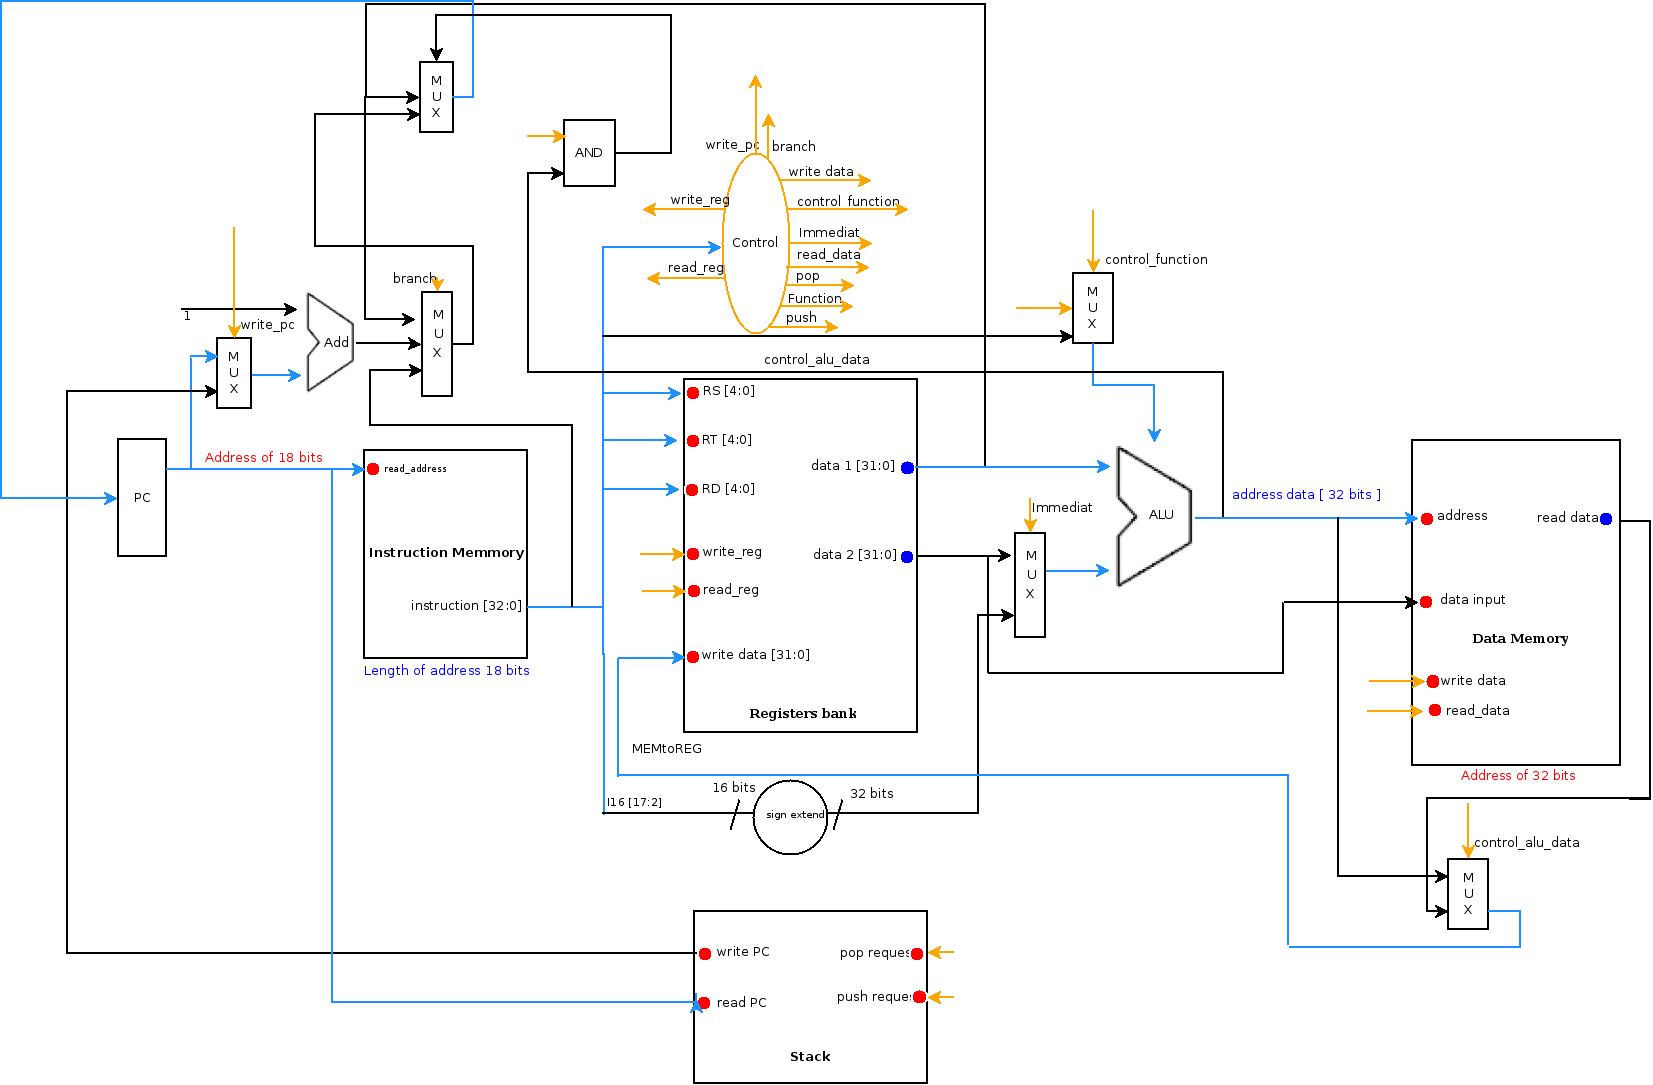
\includegraphics[width=\textwidth]{./pictures/datapath/DataPath.png}
      	\end{figure}
\end{landscape}
% Optional bibliography section
% To use bibliograpy, first provide the ipprocess.bib file on the root folder.
% \bibliographystyle{ieeetr}
% \bibliography{ipprocess}

\end{document}
